\documentclass[conference]{IEEEtran}

% ── Paquetes ──────────────────────────────────────────────────────
\usepackage[utf8]{inputenc}
\usepackage[spanish,english]{babel}
\usepackage{amsmath,amssymb}
\usepackage{graphicx}
\usepackage{booktabs}
\usepackage{hyperref}
\usepackage{float}
\usepackage{multirow}
\usepackage{array}
\usepackage{subcaption}
\usepackage{xcolor}
\usepackage{balance}

\hypersetup{
    colorlinks=true,
    urlcolor=blue,
    linkcolor=black,
    citecolor=blue
}

\hyphenation{op-tical net-works semi-conduc-tor IEEEtran}

\begin{document}

% ══════════════════════════════════════════════════════════════════
%  TÍTULO Y AUTORES
% ══════════════════════════════════════════════════════════════════
\selectlanguage{spanish}

\title{\LARGE Detecci\'{o}n de n\'{o}dulos pulmonares en radiograf\'{i}as de t\'{o}rax mediante ensemble de detectores con preentrenamiento radiol\'{o}gico: del modelo al prototipo hospitalario}

\author{
\IEEEauthorblockN{Antonio Contesti Coll, Marc Link Cladera}
\IEEEauthorblockA{
Grado en Ingenier\'{i}a Inform\'{a}tica \\
Universitat de les Illes Balears (UIB) \\
Supervisor: Miquel Mir\'{o} Nicolau
}
}

\maketitle

% ══════════════════════════════════════════════════════════════════
%  ABSTRACT (en inglés)
% ══════════════════════════════════════════════════════════════════
\selectlanguage{english}
\begin{abstract}
Early detection of pulmonary nodules in chest X-rays (CXR) remains a critical
clinical challenge due to the small size and low contrast of lesions against
overlapping anatomical structures. This work presents a comprehensive study of
deep learning techniques applied to both binary classification and spatial
detection of pulmonary nodules, using the NODE21 challenge as a common
evaluation benchmark. For classification, we evaluate six architectures
including a baseline CNN, ResNet18, DenseNet121/169, and EfficientNet-B0/B3,
and propose a multichannel representation (Original + CLAHE + Canny + Unsharp
Mask) that achieves 98.07\% accuracy with near-zero false negatives. For
detection, we compare Faster R-CNN with COCO and VinDr-CXR pretraining,
RetinaNet, YOLOv8s, and the recent YOLO26s. We demonstrate that radiological
domain pretraining (VinDr-CXR) is the single most determinant factor for
detection performance. Our main contribution is a Weighted Box Fusion (WBF)
ensemble combining Faster R-CNN VinDr and YOLOv8s, which achieves a NODE21
score of 0.9391 and a Competition Metric of 94.47\%, surpassing the original
NODE21 winner (Behrendt et al., CM=83.90\%) with only 2 models instead of 21.
We identify and quantify a data leakage artifact (+6.7 points inflation) caused
by offline augmentations, and demonstrate the critical impact of score
thresholding on FROC evaluation (+40 NODE21 points). Finally, we present a
fully functional hospital prototype with real-time GPU inference (~81\,ms per
image), an interactive web viewer, and a prospective validation module that
enables radiologists to correct predictions and export validated datasets for
continuous model improvement.
\end{abstract}

\selectlanguage{spanish}

% ══════════════════════════════════════════════════════════════════
%  I. INTRODUCCIÓN
% ══════════════════════════════════════════════════════════════════
\section{Introducci\'{o}n}

El c\'{a}ncer de pulm\'{o}n es la principal causa de mortalidad por c\'{a}ncer
a nivel mundial, y la detecci\'{o}n precoz de n\'{o}dulos pulmonares
constituye un factor determinante para mejorar las tasas de supervivencia. Las
radiograf\'{i}as de t\'{o}rax (CXR) representan la modalidad de imagen m\'{a}s
accesible y frecuente en la pr\'{a}ctica cl\'{i}nica; sin embargo, la
detecci\'{o}n de n\'{o}dulos en CXR resulta especialmente exigente debido a la
superposici\'{o}n de estructuras anat\'{o}micas, el reducido tama\~{n}o de las
lesiones y la variabilidad en las condiciones de adquisici\'{o}n. Estudios
previos indican que incluso radi\'{o}logos experimentados pueden pasar por alto
entre un 20\% y un 30\% de los n\'{o}dulos visibles en CXR, lo que subraya la
necesidad de herramientas de apoyo al diagn\'{o}stico basadas en inteligencia
artificial.

El reto NODE21~\cite{behrendt2023node21,node21challenge} proporciona un
benchmark estandarizado para evaluar m\'{e}todos de detecci\'{o}n de
n\'{o}dulos en CXR, con 4\,882 radiograf\'{i}as y 1\,476 anotaciones de
\textit{bounding boxes}. El dataset procede de cuatro fuentes p\'{u}blicas
(JSRT, PadChest, ChestX-ray14, Open-I) con una prevalencia del 23\% de
im\'{a}genes con n\'{o}dulos. La soluci\'{o}n ganadora de Behrendt et
al.~\cite{behrendt2023node21} emplea un ensemble de 21 modelos (5
arquitecturas $\times$ 5 folds) y alcanza una Competition Metric (CM) del
83.90\%.

El presente trabajo aborda el problema desde dos perspectivas complementarias:
en primer lugar, la clasificaci\'{o}n binaria (presencia/ausencia de
n\'{o}dulos) como tarea de \textit{screening}, y en segundo lugar, la
detecci\'{o}n espacial mediante \textit{bounding boxes} para localizaci\'{o}n
cl\'{i}nica precisa. Adem\'{a}s, se desarrolla un prototipo hospitalario
funcional que integra los mejores modelos en un sistema \textit{end-to-end} con
validaci\'{o}n prospectiva por radi\'{o}logos.

Las contribuciones principales son:

\begin{enumerate}
\item Un estudio exhaustivo de clasificaci\'{o}n binaria con 6 arquitecturas y
una innovaci\'{o}n multicanal (Original + CLAHE + Canny + Unsharp) que alcanza
el 98.07\% de accuracy con falsos negativos pr\'{a}cticamente nulos, junto con
un estudio de ablaci\'{o}n que identifica CLAHE como el componente clave.
\item Un ensemble WBF de solo 2 detectores (Faster R-CNN VinDr + YOLOv8s) que
obtiene un NODE21 score de 0.9391 y CM=94.47\%, superando ampliamente al
ganador NODE21 (CM=83.90\%) con un orden de magnitud menos de modelos.
\item La identificaci\'{o}n y cuantificaci\'{o}n de un artefacto de
\textit{data leakage} (+6.7 puntos de inflaci\'{o}n) causado por
augmentaciones offline no agrupadas, as\'{i} como la demostraci\'{o}n del
impacto cr\'{i}tico del \textit{score threshold} (+40 puntos NODE21).
\item Un prototipo hospitalario funcional \textit{end-to-end} con inferencia
GPU en tiempo real ($\sim$81\,ms por imagen) y un m\'{o}dulo de validaci\'{o}n
prospectiva que permite a los radi\'{o}logos corregir predicciones y exportar
datasets validados para mejora continua del modelo.
\end{enumerate}

El resto del art\'{i}culo se organiza como sigue: la Secci\'{o}n~II revisa
el trabajo relacionado; la Secci\'{o}n~III describe los materiales y
m\'{e}todos; la Secci\'{o}n~IV presenta los resultados experimentales; la
Secci\'{o}n~V detalla la herramienta hospitalaria; la Secci\'{o}n~VI discute
los hallazgos; y la Secci\'{o}n~VII concluye con las direcciones de trabajo
futuro.


% ══════════════════════════════════════════════════════════════════
%  II. TRABAJO RELACIONADO
% ══════════════════════════════════════════════════════════════════
\section{Trabajo relacionado}

\textbf{NODE21 y detecci\'{o}n de n\'{o}dulos.}
El reto NODE21~\cite{node21challenge} estandariza la evaluaci\'{o}n de
detecci\'{o}n de n\'{o}dulos pulmonares en CXR mediante la curva FROC
(\textit{Free-Response Receiver Operating Characteristic}) y una m\'{e}trica
compuesta CM = $0.75 \times \text{AUROC} + 0.25 \times \text{NODE21}$.
Behrendt et al.~\cite{behrendt2023node21} propusieron un enfoque
sistem\'{a}tico basado en Faster R-CNN con preentrenamiento en VinDr-CXR,
combinando cinco arquitecturas de backbone (ResNet50-FPN, ResNet101-FPN, y
variantes) en un ensemble de 21 modelos mediante 5-fold cross-validation,
obteniendo CM=83.90\% en el test set oficial.

\textbf{Preentrenamiento en dominio radiol\'{o}gico.}
VinDr-CXR~\cite{vindrcxr} proporciona 18\,000 radiograf\'{i}as de t\'{o}rax
anotadas por radi\'{o}logos expertos con 14 hallazgos radiol\'{o}gicos locales
(incluyendo n\'{o}dulos, masas, opacidades, cardiomegalia, entre otros) y 6
diagn\'{o}sticos globales, constituyendo una de las fuentes m\'{a}s ricas de
conocimiento de dominio radiol\'{o}gico disponibles p\'{u}blicamente. Trabajos
recientes de Rehman et al.~\cite{rehman2024} y Li et al.~\cite{li2024} han
demostrado que el preentrenamiento espec\'{i}fico en dominio radiol\'{o}gico
supera consistentemente al preentrenamiento gen\'{e}rico en ImageNet/COCO,
especialmente para la detecci\'{o}n de lesiones peque\~{n}as de bajo contraste
como los n\'{o}dulos pulmonares.

\textbf{Fusi\'{o}n de detectores.}
La estrategia cl\'{a}sica para combinar m\'{u}ltiples detectores es
Non-Maximum Suppression (NMS), que selecciona la detecci\'{o}n de mayor
confianza y suprime las solapadas. Soft-NMS suaviza este proceso reduciendo
gradualmente los scores en lugar de eliminar detecciones. Weighted Box
Fusion (WBF)~\cite{solovyev2021} propone un enfoque diferente: fusiona todas
las predicciones coincidentes calculando un promedio ponderado de coordenadas
y scores, lo que produce \textit{bounding boxes} m\'{a}s precisos y scores
m\'{a}s calibrados. WBF ha demostrado mejoras consistentes sobre NMS y
Soft-NMS en m\'{u}ltiples benchmarks de detecci\'{o}n de objetos,
particularmente cuando se combinan detectores con caracter\'{i}sticas
complementarias.

\textbf{Detectores modernos.}
Faster R-CNN~\cite{ren2015} representa el paradigma de dos etapas: una
Region Proposal Network (RPN) genera candidatos de regi\'{o}n que
posteriormente se clasifican y refinan. RetinaNet~\cite{lin2017focal}
introduce Focal Loss para abordar el desequilibrio extremo entre foreground
y background en detectores de una etapa. YOLOv8~\cite{jocher2023} aporta una
arquitectura \textit{anchor-free} con asignaci\'{o}n din\'{a}mica de tareas
(\textit{task-aligned assignment}) y cabezas desacopladas para
clasificaci\'{o}n y regresi\'{o}n. YOLO26~\cite{yolo26} es la versi\'{o}n
m\'{a}s reciente de Ultralytics, que incorpora STAL (\textit{Small-Target-Aware
Label Assignment}) dise\~{n}ado espec\'{i}ficamente para mejorar la
detecci\'{o}n de objetos peque\~{n}os, junto con inferencia libre de NMS,
ProgLoss y el optimizador MuSGD.


% ══════════════════════════════════════════════════════════════════
%  III. MATERIALES Y MÉTODOS
% ══════════════════════════════════════════════════════════════════
\section{Materiales y m\'{e}todos}

% ── III-A. Dataset NODE21 ─────────────────────────────────────────
\subsection{Dataset NODE21}

El conjunto NODE21~\cite{node21challenge} contiene 4\,882 radiograf\'{i}as de
t\'{o}rax procedentes de cuatro fuentes p\'{u}blicas (JSRT, PadChest,
ChestX-ray14, Open-I), de las cuales 1\,134 contienen n\'{o}dulos (1\,476
anotaciones de \textit{bounding boxes}) y 3\,748 son negativas (prevalencia del
23\%). Las im\'{a}genes se proporcionan en formato \texttt{.mha}
(\textit{MetaImage}) y fueron convertidas a PNG de $1024 \times 1024$
p\'{i}xeles tras normalizaci\'{o}n de intensidades al rango $[0, 255]$ y
correcci\'{o}n de orientaci\'{o}n para garantizar coherencia anat\'{o}mica.

Las anotaciones de \textit{bounding boxes} se proporcionan en formato COCO con
coordenadas $(x, y, w, h)$. El tama\~{n}o de los n\'{o}dulos es muy variable,
desde lesiones de pocos mil\'{i}metros hasta masas que ocupan una fracci\'{o}n
significativa del campo pulmonar, con una distribuci\'{o}n sesgada hacia
n\'{o}dulos peque\~{n}os.

\subsubsection{Distribuci\'{o}n espacial y tama\~{n}o de n\'{o}dulos}

El an\'{a}lisis de la distribuci\'{o}n espacial de los n\'{o}dulos anotados
(Fig.~\ref{fig:distribucion}) revela una concentraci\'{o}n predominante en los
campos pulmonares medios y superiores, coherente con la distribuci\'{o}n
cl\'{i}nica conocida de los n\'{o}dulos pulmonares. El an\'{a}lisis de
tama\~{n}o muestra que la mayor\'{i}a de los n\'{o}dulos ocupan menos del 5\%
del \'{a}rea de la imagen, confirmando la dificultad intr\'{i}nseca de la tarea
de detecci\'{o}n (Fig.~\ref{fig:tamano}). Esta distribuci\'{o}n sesgada hacia
n\'{o}dulos peque\~{n}os tiene implicaciones directas en el dise\~{n}o del
sistema: justifica la elecci\'{o}n de resoluci\'{o}n $1024 \times 1024$ (para
preservar detalles finos), el uso de un IoU threshold bajo (0.2 en NODE21, vs.\
0.5 en COCO), y motiv\'{o} la evaluaci\'{o}n de YOLO26 con STAL.

\begin{figure}[t]
\centering
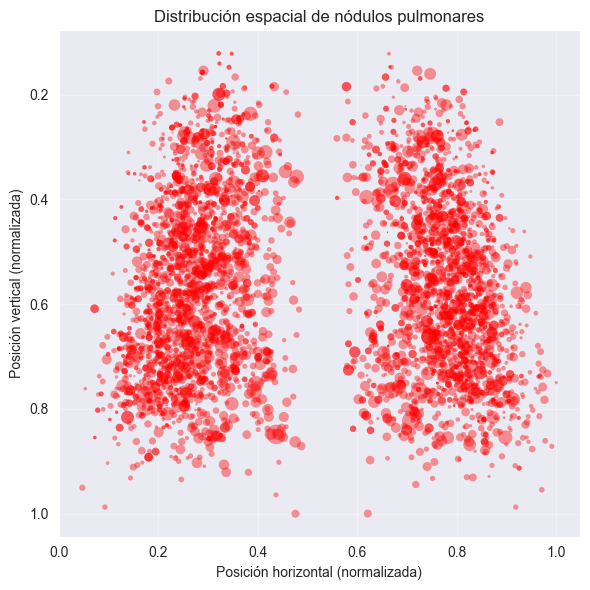
\includegraphics[width=\columnwidth]{distribucion_nodulos.png}
\caption{Distribuci\'{o}n espacial de los n\'{o}dulos anotados en el dataset
NODE21. Se observa concentraci\'{o}n en los campos pulmonares medios y
superiores.}
\label{fig:distribucion}
\end{figure}

\begin{figure}[t]
\centering
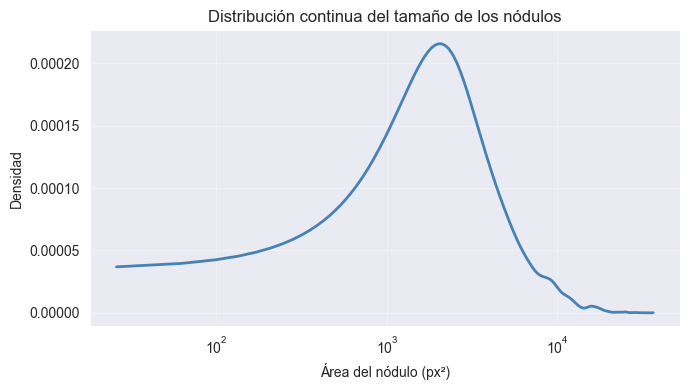
\includegraphics[width=\columnwidth]{distribucion_tamao_nodulo.png}
\caption{Distribuci\'{o}n de tama\~{n}o de los n\'{o}dulos en NODE21. La
mayor\'{i}a son lesiones peque\~{n}as ($<$5\% del \'{a}rea de imagen),
confirmando la dificultad de la tarea.}
\label{fig:tamano}
\end{figure}

Para la divisi\'{o}n train/validaci\'{o}n se utiliz\'{o}
\texttt{StratifiedGroupKFold} con 5 folds, estratificando por clase
(positivo/negativo) y agrupando por imagen base. Esta agrupaci\'{o}n es
cr\'{i}tica para evitar \textit{data leakage} cuando se utilizan
augmentaciones offline, como se detalla en la
Secci\'{o}n~\ref{sec:leakage}.


% ── III-B. Clasificación binaria ──────────────────────────────────
\subsection{Fase de clasificaci\'{o}n binaria}
\label{sec:clasificacion}

La primera fase del trabajo se centr\'{o} en la clasificaci\'{o}n binaria
(presencia/ausencia de n\'{o}dulos) como tarea de \textit{screening}. Se
evaluaron 6 arquitecturas progresivamente m\'{a}s sofisticadas:

\textbf{SimpleCNN} (baseline): red convolucional de 3 bloques entrenada desde
cero, sin \textit{transfer learning}. Opera sobre im\'{a}genes de $224 \times
224$ con un canal de entrada. Entrenada durante 10 \'{e}pocas con Adam y
Cross-Entropy. Establece una l\'{i}nea base de 79.04\% de accuracy.

\textbf{ResNet18}: arquitectura con conexiones residuales, inicializada con
pesos ImageNet. Capas convolucionales congeladas, solo se entrena el
clasificador final. Mejora la accuracy a 81.05\% pero con un recall de la
clase positiva muy bajo (45.37\%), indicando una fuerte inclinaci\'{o}n hacia
la clase mayoritaria.

\textbf{DenseNet121/169}: arquitecturas con conexiones densas que facilitan la
reutilizaci\'{o}n de caracter\'{i}sticas. DenseNet169 alcanza 85.55\% de
accuracy y 70.93\% de recall positivo, demostrando la ventaja de redes
m\'{a}s profundas con conectividad densa para imagen m\'{e}dica.

\textbf{EfficientNet-B0/B3}: arquitecturas basadas en escalado compuesto
(\textit{compound scaling}). EfficientNet-B0 ofrece el mejor compromiso
global: 86.03\% accuracy y 73.48\% recall positivo. EfficientNet-B3, pese a
mayor capacidad, muestra inferior recall (66.13\%), posiblemente por
sobreajuste en un dataset relativamente peque\~{n}o.

La Tabla~\ref{tab:clasificacion} resume los resultados. Todas las im\'{a}genes
se normalizaron a $224 \times 224$, replicando el canal gris a 3 canales RGB.
La divisi\'{o}n fue 80\%/20\% train/test.

\begin{table}[t]
\caption{Comparaci\'{o}n de modelos de clasificaci\'{o}n binaria sobre NODE21}
\label{tab:clasificacion}
\centering
\footnotesize
\setlength{\tabcolsep}{3pt}
\begin{tabular}{lcccc}
\toprule
\textbf{Modelo} & \textbf{Acc.(\%)} & \textbf{Prec.(\%)} & \textbf{Rec.+(\%)} & \textbf{F1+(\%)} \\
\midrule
SimpleCNN        & 79.04 & 64.87 & 65.50 & 65.18 \\
ResNet18         & 81.05 & 84.02 & 45.37 & 58.92 \\
DenseNet121      & 84.59 & 76.21 & 70.61 & 73.30 \\
DenseNet169      & 85.55 & 78.79 & 70.93 & 74.65 \\
EfficientNet-B0  & \textbf{86.03} & 77.00 & \textbf{73.48} & \textbf{75.20} \\
EfficientNet-B3  & 85.17 & 79.50 & 66.13 & 72.22 \\
\bottomrule
\end{tabular}
\end{table}

La Fig.~\ref{fig:comparacion_clasif} visualiza las m\'{e}tricas principales
de los 6 modelos, evidenciando la progresi\'{o}n de rendimiento desde el
\textit{baseline} hasta las arquitecturas con escalado compuesto.

\begin{figure}[t]
\centering
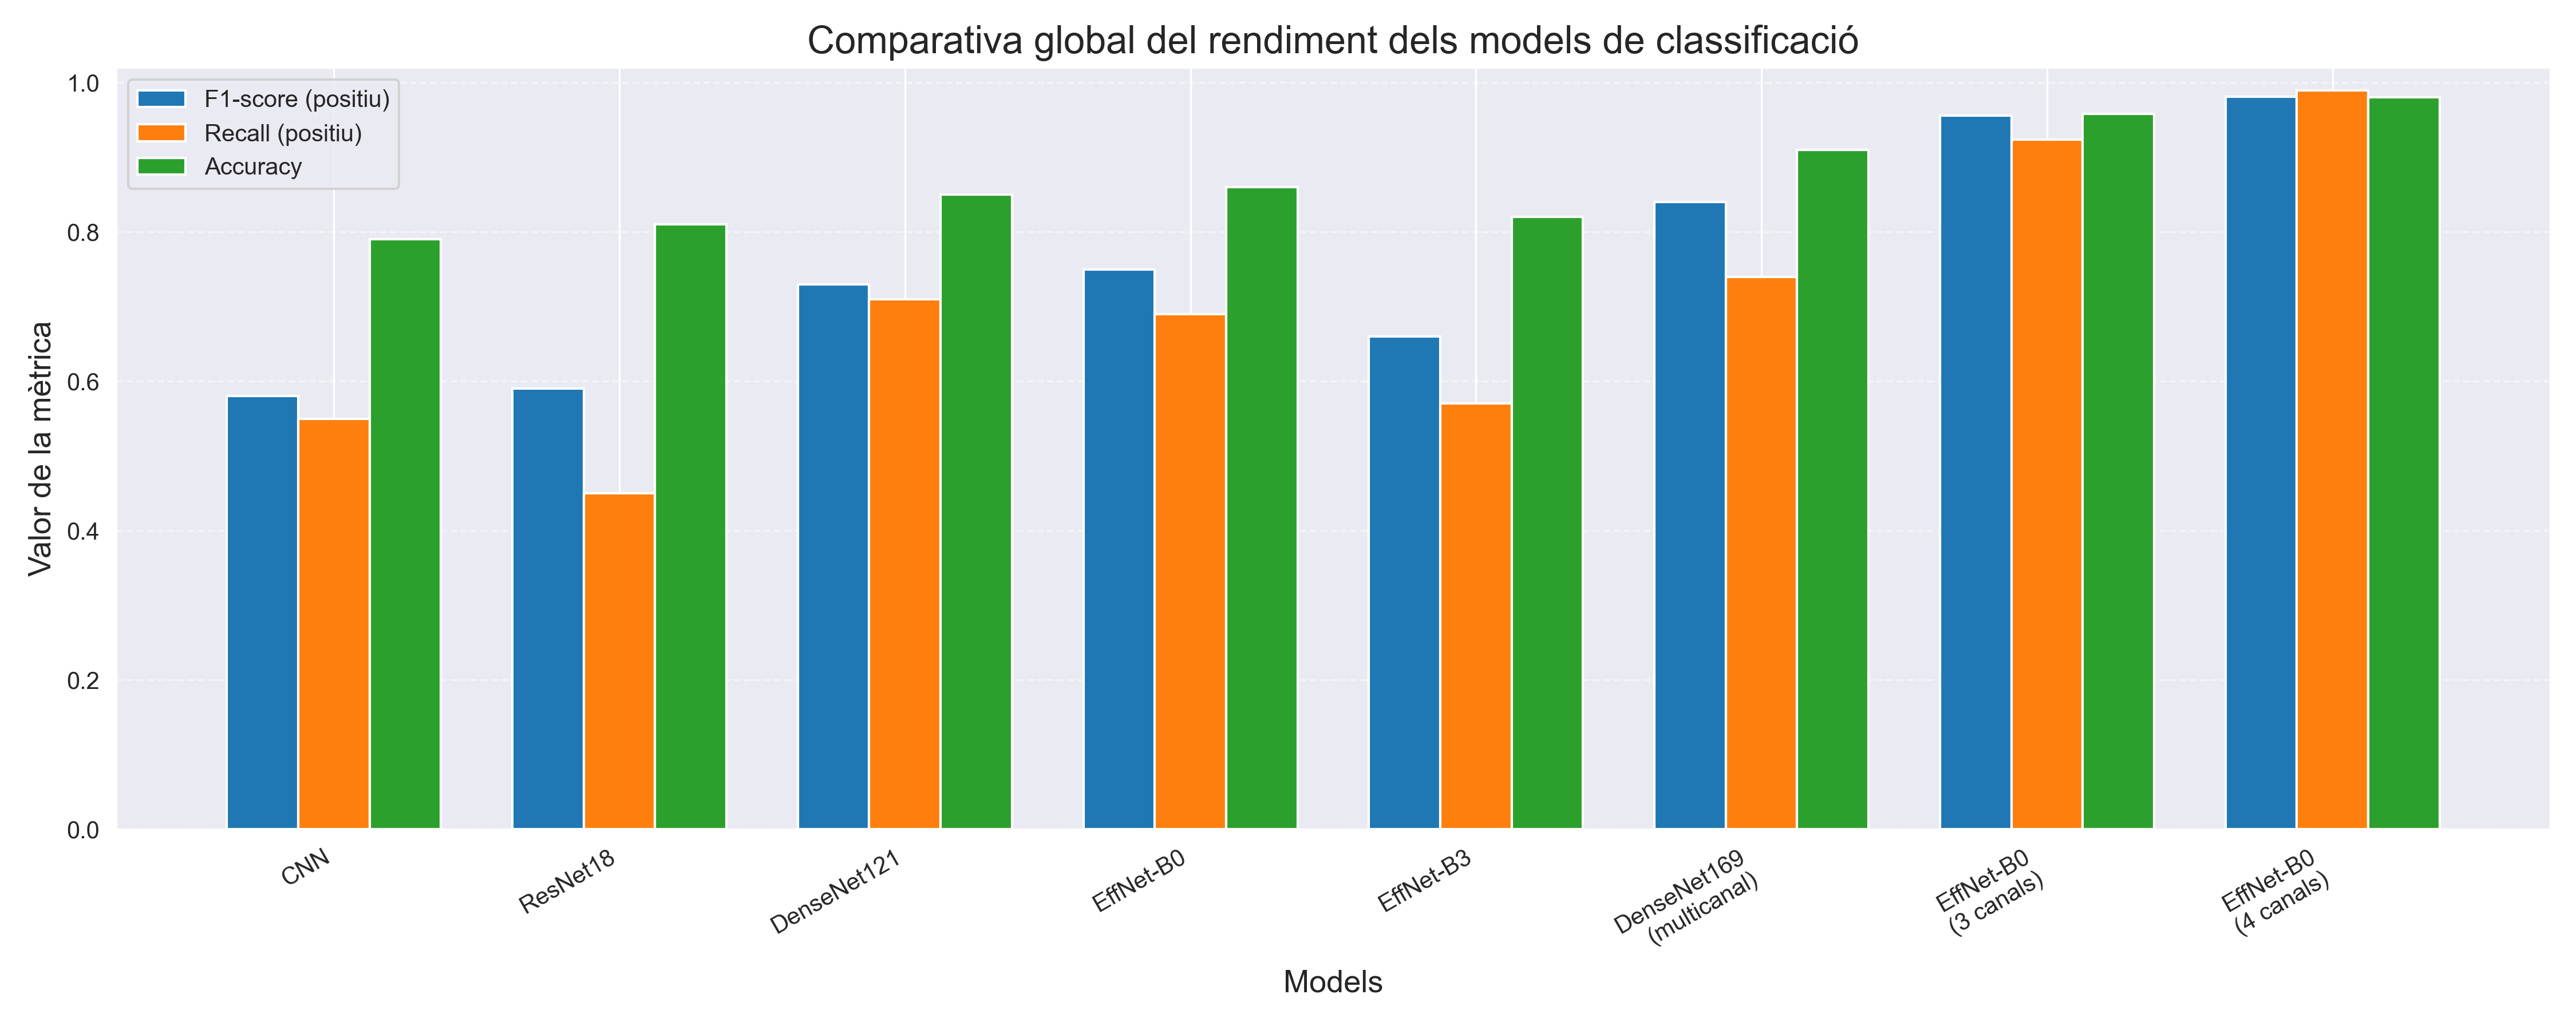
\includegraphics[width=\columnwidth]{comparativa_models_classificacio.png}
\caption{Comparaci\'{o}n de m\'{e}tricas de los 6 modelos de
clasificaci\'{o}n. EfficientNet-B0 ofrece el mejor equilibrio entre accuracy
y recall positivo.}
\label{fig:comparacion_clasif}
\end{figure}

Aunque EfficientNet-B0 obtiene el mejor resultado est\'{a}ndar, ninguno de los
6 modelos supera el 73\% de recall para la clase positiva. En un contexto
cl\'{i}nico de \textit{screening}, donde un falso negativo puede suponer un
retraso en el diagn\'{o}stico de c\'{a}ncer de pulm\'{o}n, este nivel de
recall resulta claramente insuficiente.

\subsubsection{Innovaci\'{o}n multicanal}

Para superar esta limitaci\'{o}n, se propuso una representaci\'{o}n
multicanal que enriquece la informaci\'{o}n de entrada al modelo. En lugar de
alimentar la red con la imagen original (o su r\'{e}plica a 3 canales RGB), se
construye un tensor de 4 canales donde cada canal aporta informaci\'{o}n
complementaria (Fig.~\ref{fig:multicanal}):

\begin{enumerate}
\item \textbf{Canal 1 --- Original}: imagen normalizada al rango $[0, 1]$.
\item \textbf{Canal 2 --- CLAHE}: ecualizaci\'{o}n adaptativa de histograma con
l\'{i}mite de contraste (\textit{Contrast Limited Adaptive Histogram
Equalization}), que realza el contraste local de los n\'{o}dulos respecto al
fondo pulmonar sin amplificar el ruido global.
\item \textbf{Canal 3 --- Canny}: detecci\'{o}n de bordes que delimita los
contornos de las estructuras anat\'{o}micas y, potencialmente, de los
n\'{o}dulos.
\item \textbf{Canal 4 --- Unsharp Mask}: enfatiza texturas finas y detalles de
alta frecuencia que pueden corresponder a la textura caracter\'{i}stica de los
n\'{o}dulos.
\end{enumerate}

\begin{figure}[t]
\centering
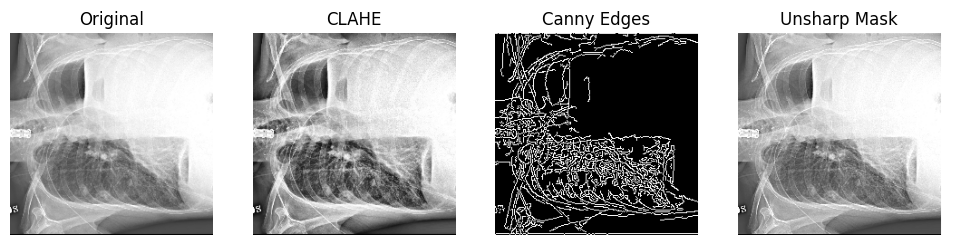
\includegraphics[width=\columnwidth]{rx_4_capas.png}
\caption{Pipeline multicanal: la imagen original se procesa para generar 4
canales complementarios (Original, CLAHE, Canny, Unsharp Mask) que se apilan
como entrada al modelo de clasificaci\'{o}n.}
\label{fig:multicanal}
\end{figure}

Se adapt\'{o} EfficientNet-B0 modificando la primera capa convolucional para
aceptar 4 canales de entrada. Adicionalmente, se reequilibr\'{o} el dataset
mediante augmentaci\'{o}n dirigida de la clase minoritaria (positivos),
aplicando transformaciones geom\'{e}tricas y fotom\'{e}tricas suaves. Con esta
configuraci\'{o}n se alcanz\'{o} una accuracy del \textbf{98.07\%} con un
recall del 98.93\% para la clase positiva (solo 1.1\% de falsos negativos) y
2.8\% de falsos positivos.

\subsubsection{Estudio de ablaci\'{o}n}

El an\'{a}lisis de ablaci\'{o}n (Tabla~\ref{tab:ablacion}) permite cuantificar
la contribuci\'{o}n de cada componente del pipeline multicanal. Se evaluaron
9 configuraciones variando el n\'{u}mero de canales (1--4) y el balanceo del
dataset.

\begin{table}[t]
\caption{Estudio de ablaci\'{o}n del pipeline multicanal. ``bal.'' indica
dataset balanceado mediante augmentaci\'{o}n dirigida.}
\label{tab:ablacion}
\centering
\footnotesize
\setlength{\tabcolsep}{2pt}
\begin{tabular}{clcccc}
\toprule
\textbf{Ch} & \textbf{Configuraci\'{o}n} & \textbf{Acc.(\%)} & \textbf{Rec.+(\%)} & \textbf{FN} & \textbf{FP} \\
\midrule
1 & Original              & 96.67 & 95.73 & 32 & 18 \\
1 & Canny                 & 91.73 & 84.78 & 114 & 10 \\
1 & Unsharp               & 96.73 & 95.46 & 34 & 15 \\
2 & Orig. + CLAHE         & 98.13 & 99.33 & 5 & 23 \\
\textbf{2} & \textbf{Orig. + CLAHE (bal.)} & \textbf{98.84} & \textbf{99.55} & \textbf{4} & \textbf{15} \\
3 & O.+CLAHE+Canny        & 97.13 & 96.93 & 23 & 20 \\
3 & O.+CLAHE+Unsharp (bal.) & 98.84 & 99.33 & 6 & 13 \\
4 & O.+C.+Ca.+U.          & 98.13 & 98.00 & 15 & 13 \\
4 & O.+C.+Ca.+U. (bal.)   & 98.35 & 98.21 & 16 & 11 \\
\bottomrule
\end{tabular}
\end{table}

Los resultados revelan tres hallazgos principales: (1)~CLAHE es el componente
m\'{a}s determinante, responsable del salto de $\sim$96.7\% a $\sim$98.1\%
de accuracy; (2)~el balanceo del dataset aporta una mejora adicional,
reduciendo falsos positivos sin sacrificar recall; (3)~la adici\'{o}n de
canales Canny y Unsharp no mejora consistentemente el rendimiento, y en
algunos casos introduce ruido. La configuraci\'{o}n \'{o}ptima es
\textbf{Original + CLAHE con dataset balanceado}: 98.84\% accuracy, 99.55\%
recall positivo y solo 4 falsos negativos, resultando especialmente apropiada
para escenarios de \textit{screening} cl\'{i}nico.

\subsubsection{Explicabilidad con Integrated Gradients}

Para validar que los modelos multicanal enfocan su atenci\'{o}n en regiones
cl\'{i}nicamente relevantes, se aplic\'{o} \textit{Integrated Gradients}
(IG) como t\'{e}cnica de explicabilidad. Los mapas de atribuci\'{o}n
resultantes (Fig.~\ref{fig:ig}) confirman que el modelo concentra su
atenci\'{o}n en las zonas del par\'{e}nquima pulmonar donde se localizan los
n\'{o}dulos, con mayor activaci\'{o}n en el canal CLAHE, lo que refuerza la
hip\'{o}tesis de que el realce de contraste local facilita la
discriminaci\'{o}n de estas lesiones.

\begin{figure}[t]
\centering
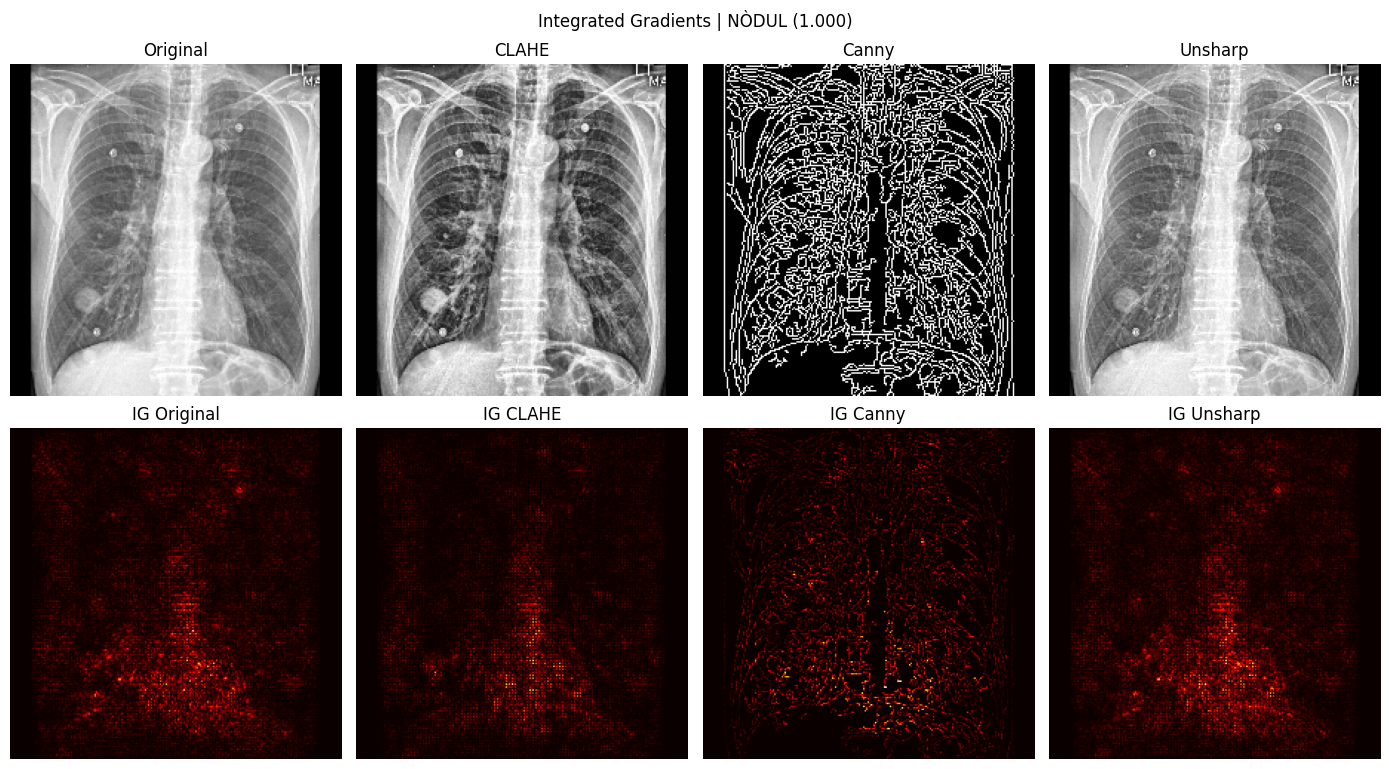
\includegraphics[width=\columnwidth]{ig_multicanal_example.png}
\caption{Mapas de atribuci\'{o}n Integrated Gradients sobre el pipeline
multicanal. La atenci\'{o}n del modelo se concentra en las regiones
pulmonares con n\'{o}dulos, especialmente en el canal CLAHE.}
\label{fig:ig}
\end{figure}


% ── III-C. Detección de nódulos ───────────────────────────────────
\subsection{Detecci\'{o}n de n\'{o}dulos con \textit{bounding boxes}}

La segunda fase del trabajo se centra en la detecci\'{o}n espacial de
n\'{o}dulos, que proporciona no solo la presencia sino la localizaci\'{o}n
precisa de cada lesi\'{o}n. Se evaluaron 4 detectores agrupados en dos
paradigmas: detectores de dos etapas (Faster R-CNN) y de una etapa
(YOLOv8, YOLO26).

\subsubsection{Faster R-CNN con pretraining COCO}

Como l\'{i}nea base de detecci\'{o}n, se evalu\'{o} Faster
R-CNN~\cite{ren2015} con backbone ResNet50-FPN preentrenado en COCO. Se
probaron dos variantes: (a)~backbone completamente congelado, entrenando solo
las cabezas de RPN y clasificaci\'{o}n/regresi\'{o}n; y (b)~\textit{fine-tuning}
parcial descongelando las \'{u}ltimas capas del backbone. Los resultados
(NODE21 $\approx$ 0.63--0.66) confirman que el preentrenamiento en im\'{a}genes
naturales es insuficiente para la detecci\'{o}n de n\'{o}dulos pulmonares, con
sensibilidades particularmente bajas en reg\'{i}menes estrictos (37.2\% a
0.25~FP/imagen).

\subsubsection{Faster R-CNN con pretraining VinDr-CXR}

Se utiliz\'{o} Faster R-CNN con backbone ResNet50-FPN, inicializado con pesos
preentrenados por Behrendt et al.~\cite{behrendt2023node21} sobre
VinDr-CXR~\cite{vindrcxr} (14 hallazgos radiol\'{o}gicos). La carga de pesos
se realiz\'{o} mediante mapeo secuencial de \textit{keys} entre la
arquitectura del modelo publicado y la implementaci\'{o}n est\'{a}ndar de
\texttt{torchvision}, eliminando la cabeza de clasificaci\'{o}n original (14
clases VinDr) e inicializando una nueva cabeza para detecci\'{o}n binaria (1
clase: n\'{o}dulo).

La estrategia de congelaci\'{o}n fue selectiva: las capas 1--3 del backbone
(que codifican caracter\'{i}sticas gen\'{e}ricas de bajo y medio nivel) se
congelaron, manteniendo entrenables la capa~4 (caracter\'{i}sticas de alto
nivel), el FPN completo y las cabezas de detecci\'{o}n (32.8M de 41.3M
par\'{a}metros totales). Esta estrategia permite adaptar las
representaciones de alto nivel al dominio espec\'{i}fico de NODE21
conservando el conocimiento radiol\'{o}gico aprendido de VinDr-CXR.

La entrada consiste en im\'{a}genes en escala de grises replicadas a 3 canales,
de $1024 \times 1024$ p\'{i}xeles. Se entren\'{o} con AdamW (lr=$10^{-4}$,
weight decay=$10^{-4}$), \textit{batch size}~2 y 40 \'{e}pocas. Se exploraron
variantes con CBAM (\textit{Convolutional Block Attention Module}) insertado en
el backbone, y con Focal Loss como funci\'{o}n de p\'{e}rdida alternativa a la
Cross-Entropy est\'{a}ndar, que mostraron comportamiento estable pero sin
mejoras sustanciales sobre la configuraci\'{o}n base ya optimizada.

\subsubsection{YOLOv8s}

YOLOv8s~\cite{jocher2023} es un detector \textit{anchor-free} de una sola
etapa con asignaci\'{o}n din\'{a}mica de tareas (\textit{task-aligned
assignment}) y cabezas desacopladas para clasificaci\'{o}n y regresi\'{o}n de
\textit{bounding boxes}. Se utiliz\'{o} la variante \texttt{s} (peque\~{n}a,
11.2M par\'{a}metros) preentrenada en COCO.

El entrenamiento se realiz\'{o} a resoluci\'{o}n $1024 \times 1024$ (frente a
los 640 p\'{i}xeles por defecto) para mejorar la detecci\'{o}n de
n\'{o}dulos peque\~{n}os. La augmentaci\'{o}n se limit\'{o} estrictamente a
\textit{flip} horizontal, desactivando \textit{mosaic}, \textit{mixup},
transformaciones de color y recortes aleatorios, ya que estas t\'{e}cnicas
pueden distorsionar la apariencia radiol\'{o}gica y generar artefactos
incompatibles con la anatom\'{i}a tor\'{a}cica. Se entren\'{o} con AdamW
(lr=$10^{-4}$), 100 \'{e}pocas y \textit{early stopping} con patience de 20.

\subsubsection{YOLO26s}

YOLO26~\cite{yolo26} es la versi\'{o}n m\'{a}s reciente de la familia
Ultralytics, que incorpora STAL (\textit{Small-Target-Aware Label Assignment}),
un m\'{e}todo de asignaci\'{o}n de etiquetas dise\~{n}ado espec\'{i}ficamente
para mejorar la detecci\'{o}n de objetos peque\~{n}os. Adem\'{a}s, incluye
inferencia libre de NMS (\textit{NMS-free}), ProgLoss (p\'{e}rdida progresiva)
y el optimizador MuSGD. Se evalu\'{o} con la misma configuraci\'{o}n de
entrenamiento que YOLOv8s (resoluci\'{o}n 1024, augmentaci\'{o}n conservadora)
para asegurar una comparaci\'{o}n justa.

\subsubsection{Ensemble WBF (Weighted Box Fusion)}
\label{sec:wbf}

Weighted Box Fusion~\cite{solovyev2021} fusiona las predicciones de
m\'{u}ltiples detectores de la siguiente manera: para cada grupo de
\textit{bounding boxes} coincidentes (IoU $\geq$ umbral), calcula las
coordenadas finales como el promedio ponderado de las coordenadas de los
boxes contribuyentes, y el score final como la suma ponderada de los scores
individuales. A diferencia de NMS (que descarta boxes) y Soft-NMS (que reduce
scores), WBF \textbf{utiliza todas las predicciones} para generar boxes
m\'{a}s precisos.

Nuestro ensemble combina Faster R-CNN VinDr y YOLOv8s con los siguientes
hiperpar\'{a}metros:
\begin{itemize}
\item \textbf{Pesos}: $[0.90, 0.91]$, proporcionales al NODE21 score individual
de cada modelo.
\item \textbf{IoU threshold}: 0.2 (consistente con el criterio oficial NODE21).
\item \textbf{\texttt{skip\_box\_thr}}: 0.05 (descarta detecciones con score
$<$ 0.05 antes de la fusi\'{o}n).
\end{itemize}

La complementariedad de ambos modelos es la raz\'{o}n fundamental del
\'{e}xito del ensemble: Faster R-CNN con pretraining radiol\'{o}gico aporta
alto recall con baja tasa de falsos positivos en reg\'{i}menes estrictos
(conocimiento radiol\'{o}gico de dominio), mientras que YOLOv8s contribuye con
alta sensibilidad global y eficiencia computacional (arquitectura moderna
\textit{anchor-free}).


% ── III-D. Métricas ──────────────────────────────────────────────
\subsection{M\'{e}tricas de evaluaci\'{o}n}

Se utilizan las m\'{e}tricas oficiales del reto NODE21:
\begin{itemize}
\item \textbf{NODE21 score}: media de sensibilidad a niveles de FP/imagen
$\in \{0.25, 0.5, 1, 2, 4, 8\}$ en la curva FROC. Define:
\begin{equation}
\text{NODE21} = \frac{1}{6}\sum_{i \in \{0.25, 0.5, 1, 2, 4, 8\}} \text{Sens}(i)
\end{equation}
\item \textbf{AUROC}: \'{a}rea bajo la curva ROC a nivel de imagen (detecci\'{o}n
de presencia vs.\ ausencia de n\'{o}dulos).
\item \textbf{Competition Metric (CM)}:
\begin{equation}
\text{CM} = 0.75 \times \text{AUROC} + 0.25 \times \text{NODE21}
\end{equation}
\item \textbf{IoU threshold}: 0.2 (oficial NODE21), m\'{a}s permisivo que el
est\'{a}ndar COCO (0.5) debido al tama\~{n}o reducido de los n\'{o}dulos.
\item \textbf{Score threshold}: 0.005 para evaluaci\'{o}n FROC (ver
Secci\'{o}n~\ref{sec:threshold}).
\end{itemize}


% ── III-E. Análisis del código de referencia ─────────────────────
\subsection{An\'{a}lisis del c\'{o}digo de referencia}

Un aspecto significativo del trabajo fue la revisi\'{o}n del c\'{o}digo fuente
publicado por Behrendt et al.~\cite{behrendt2023node21}. De las $\sim$3\,000
l\'{i}neas de c\'{o}digo, se identificaron 26 \textit{bugs} e
incompatibilidades: (1)~uso de APIs obsoletas de PyTorch Lightning que
impiden la ejecuci\'{o}n con Lightning~2.x; (2)~dependencias no declaradas y
versiones incompatibles; (3)~errores en la l\'{o}gica de evaluaci\'{o}n FROC.
Estos problemas hac\'{i}an el c\'{o}digo inutilizable para reproducci\'{o}n
directa. De la implementaci\'{o}n original solo se extrajeron las ideas clave
para la carga de pesos VinDr-CXR ($\sim$20 l\'{i}neas \'{u}tiles),
reimplementando el resto del pipeline de entrenamiento, evaluaci\'{o}n e
inferencia de manera independiente con PyTorch~2.x.


% ══════════════════════════════════════════════════════════════════
%  IV. RESULTADOS
% ══════════════════════════════════════════════════════════════════
\section{Resultados}

% ── IV-A. Resultados de detección ────────────────────────────────
\subsection{Resultados principales de detecci\'{o}n}

La Tabla~\ref{tab:deteccion} presenta los resultados de todos los detectores
evaluados. Todos los scores corresponden a evaluaci\'{o}n honesta sin
\textit{data leakage} (Secci\'{o}n~\ref{sec:leakage}), con \textit{score
threshold} 0.005 (Secci\'{o}n~\ref{sec:threshold}).

\begin{table}[t]
\caption{Resultados de detecci\'{o}n de n\'{o}dulos pulmonares. Todos los
scores son honestos (sin \textit{data leakage}).}
\label{tab:deteccion}
\centering
\footnotesize
\setlength{\tabcolsep}{2.5pt}
\begin{tabular}{lcccc}
\toprule
\textbf{Modelo} & \textbf{NODE21} & \textbf{AUROC} & \textbf{CM(\%)} & \textbf{S@0.25} \\
\midrule
\textbf{Ensemble WBF} & \textbf{0.9391} & \textbf{0.9683} & \textbf{94.47} & \textbf{0.874} \\
YOLOv8s                & 0.9103 & 0.9686 & 92.83 & 0.821 \\
FRCNN VinDr            & 0.9025 & 0.9460 & 91.46 & 0.821 \\
YOLO26s                & 0.7929 & 0.9557 & 87.54 & 0.635 \\
RetinaNet (COCO)       & 0.7420 & ---    & ---   & 0.470 \\
FRCNN COCO (frozen)    & 0.6620 & ---    & ---   & 0.372 \\
FRCNN COCO (fine-tune) & 0.6300 & ---    & ---   & 0.350 \\
\bottomrule
\end{tabular}
\end{table}

El ensemble WBF obtiene el mejor rendimiento en todas las m\'{e}tricas, con un
NODE21 score de 0.9391 (+2.9 puntos sobre YOLOv8s individual) y una CM del
94.47\%. Se observan tres grupos de rendimiento claramente diferenciados:
(1)~modelos con pretraining radiol\'{o}gico + ensemble ($\geq$0.90 NODE21);
(2)~YOLO26 y RetinaNet con COCO ($\sim$0.74--0.79); y (3)~Faster R-CNN con
COCO ($\sim$0.63--0.66). El preentrenamiento VinDr-CXR marca la diferencia
m\'{a}s significativa: +24 puntos de NODE21 para el mismo Faster R-CNN.

% ── IV-B. Curvas FROC ────────────────────────────────────────────
\subsection{Curvas FROC comparativas}

La Fig.~\ref{fig:froc} muestra las curvas FROC de los detectores principales.
El ensemble WBF domina en todos los puntos de operaci\'{o}n, con una ventaja
especialmente pronunciada en el r\'{e}gimen de bajos falsos positivos
($\leq$0.5~FP/imagen), que es cl\'{i}nicamente el m\'{a}s relevante ya que en
la pr\'{a}ctica cl\'{i}nica se busca minimizar la carga de trabajo adicional
generada por falsos positivos.

\begin{figure}[t]
\centering
\includegraphics[width=\columnwidth]{ensemble.png}
\caption{Curvas FROC comparativas. El ensemble WBF (l\'{i}nea superior) domina
en todos los reg\'{i}menes de falsos positivos. La mayor ventaja se observa en
el rango cl\'{i}nicamente relevante de 0.25--1~FP/imagen.}
\label{fig:froc}
\end{figure}

% ── IV-C. Sensibilidad por nivel de FP ───────────────────────────
\subsection{Sensibilidad por nivel de falsos positivos}

La Tabla~\ref{tab:sensibilidad} detalla la sensibilidad de los tres mejores
detectores a cada nivel de falsos positivos por imagen, que son los puntos
de operaci\'{o}n utilizados para calcular el NODE21 score.

\begin{table}[t]
\caption{Sensibilidad por nivel de FP/imagen en la curva FROC}
\label{tab:sensibilidad}
\centering
\footnotesize
\setlength{\tabcolsep}{2.5pt}
\begin{tabular}{lcccccc}
\toprule
\textbf{Modelo} & \textbf{@0.25} & \textbf{@0.5} & \textbf{@1} & \textbf{@2} & \textbf{@4} & \textbf{@8} \\
\midrule
Ensemble & \textbf{.874} & \textbf{.914} & \textbf{.944} & \textbf{.960} & \textbf{.970} & \textbf{.973} \\
YOLOv8s  & .821 & .870 & .924 & .953 & .957 & .957 \\
FRCNN V. & .821 & .854 & .890 & .930 & .947 & .973 \\
\bottomrule
\end{tabular}
\end{table}

A 0.25~FP/imagen (el r\'{e}gimen m\'{a}s estricto), el ensemble alcanza 87.4\%
de sensibilidad, +5.3 puntos porcentuales (pp) sobre los modelos individuales.
A 8~FP/imagen, la sensibilidad converge al 97.3\%. Es notable que YOLOv8s
supera a FRCNN VinDr en sensibilidades intermedias (0.5--2~FP/imagen), mientras
que FRCNN VinDr iguala al ensemble a 8~FP/imagen (97.3\%), confirmando la
complementariedad de ambos modelos.

% ── IV-D. Ejemplos de detección ──────────────────────────────────
\subsection{Ejemplos de detecci\'{o}n}

La Fig.~\ref{fig:detecciones} muestra ejemplos representativos de detecciones
del ensemble WBF comparados con las anotaciones \textit{ground truth}. El
sistema detecta correctamente n\'{o}dulos de diferentes tama\~{n}os y
localizaciones, incluyendo lesiones peque\~{n}as y de bajo contraste.

\begin{figure}[t]
\centering
\begin{subfigure}[t]{0.48\columnwidth}
\centering
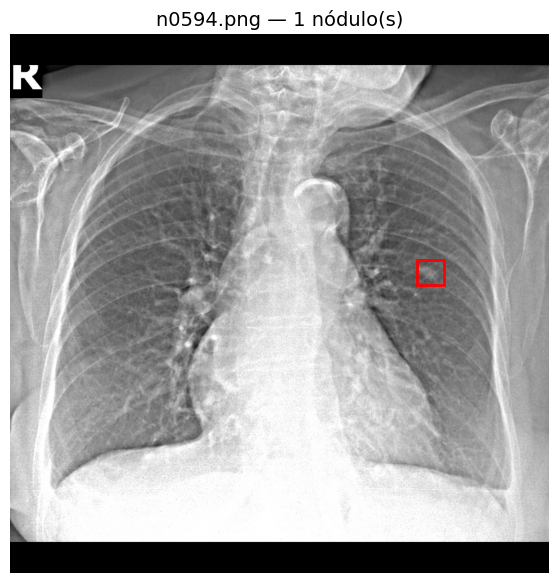
\includegraphics[width=\textwidth]{gt_example_frcnn.png}
\caption{Ground truth}
\end{subfigure}
\hfill
\begin{subfigure}[t]{0.48\columnwidth}
\centering
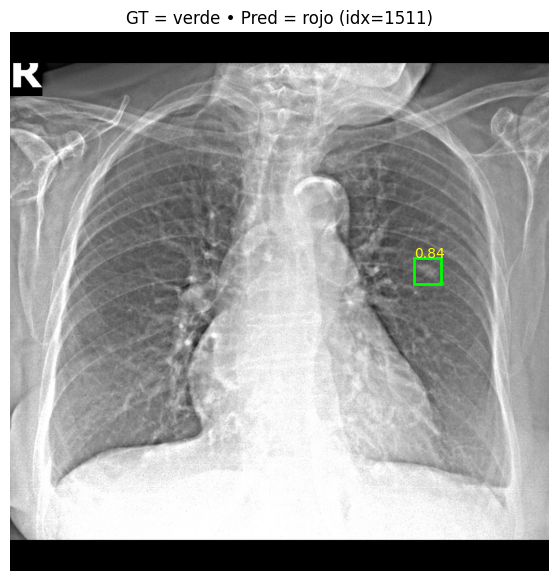
\includegraphics[width=\textwidth]{pred_example_frcnn.png}
\caption{Predicci\'{o}n ensemble}
\end{subfigure}
\caption{Ejemplo de detecci\'{o}n: (a) anotaciones \textit{ground truth} y
(b) predicciones del ensemble WBF. Los boxes verdes indican detecciones
correctas (IoU $\geq$ 0.2).}
\label{fig:detecciones}
\end{figure}


% ── IV-E. Impacto del pretraining VinDr vs COCO ──────────────────
\subsection{Impacto del pretraining radiol\'{o}gico}

La Fig.~\ref{fig:froc_vindr_coco} compara directamente las curvas FROC de
Faster R-CNN con pretraining COCO vs.\ VinDr-CXR. La diferencia es
dram\'{a}tica en todos los reg\'{i}menes de falsos positivos: a
0.25~FP/imagen, FRCNN VinDr alcanza 82.1\% de sensibilidad frente al 37.2\%
de FRCNN COCO (frozen), una mejora de $\times$2.2. Incluso comparando con la
variante COCO con \textit{fine-tuning} parcial (35.0\% a 0.25~FP/imagen), la
ventaja del pretraining radiol\'{o}gico es abrumadora. Este resultado tiene
implicaciones pr\'{a}cticas directas: sugiere que para tareas de detecci\'{o}n
en imagen m\'{e}dica, invertir en preentrenamiento de dominio es m\'{a}s
efectivo que explorar arquitecturas m\'{a}s complejas o t\'{e}cnicas de
entrenamiento m\'{a}s sofisticadas.

\begin{figure}[t]
\centering
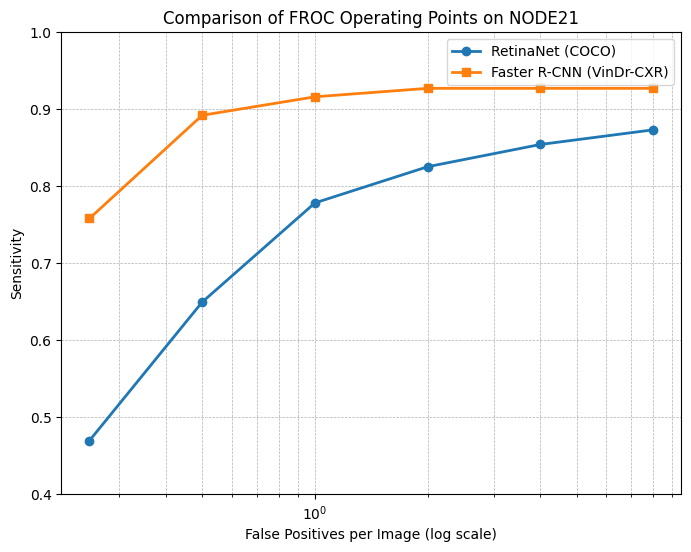
\includegraphics[width=\columnwidth]{comparison_froc_retinanet_vindr.png}
\caption{Curvas FROC comparando el impacto del dominio de preentrenamiento.
El pretraining en VinDr-CXR (dominio radiol\'{o}gico) supera ampliamente al
pretraining COCO (dominio natural) con la misma arquitectura Faster R-CNN.}
\label{fig:froc_vindr_coco}
\end{figure}


% ── IV-F. Data leakage ──────────────────────────────────────────
\subsection{Data leakage: impacto y correcci\'{o}n}
\label{sec:leakage}

Durante el desarrollo del pipeline de entrenamiento se descubri\'{o} un
artefacto de \textit{data leakage} con impacto significativo en los resultados.
El problema se origina en la augmentaci\'{o}n offline del dataset: para
mitigar el desequilibrio de clases (23\% positivos), se generaron versiones
aumentadas de las im\'{a}genes positivas (rotaciones, \textit{flips},
variaciones de contraste). Sin embargo, la divisi\'{o}n train/validaci\'{o}n
original no agrupaba estas augmentaciones con su imagen base, permitiendo que
versiones transformadas de la misma radiograf\'{i}a aparecieran
simult\'{a}neamente en train y validaci\'{o}n. Dado que las transformaciones
geom\'{e}tricas preservan la estructura espacial de los n\'{o}dulos, el modelo
pod\'{i}a ``memorizar'' patrones espec\'{i}ficos de im\'{a}genes individuales
en lugar de aprender caracter\'{i}sticas generalizables.

La Tabla~\ref{tab:leakage} cuantifica el impacto.

\begin{table}[t]
\caption{Impacto del \textit{data leakage} en Faster R-CNN VinDr}
\label{tab:leakage}
\centering
\footnotesize
\begin{tabular}{lcc}
\toprule
\textbf{Condici\'{o}n} & \textbf{NODE21} & \textbf{$\Delta$} \\
\midrule
Con leakage (split no agrupado)    & 0.9695 & ---       \\
Sin leakage (\texttt{GroupKFold})  & 0.9025 & $-$6.7 pp \\
\bottomrule
\end{tabular}
\end{table}

La correcci\'{o}n se implement\'{o} reemplazando \texttt{StratifiedKFold} por
\texttt{StratifiedGroupKFold} agrupando por identificador de imagen base, lo
que garantiza que todas las augmentaciones de una misma imagen permanezcan en
la misma partici\'{o}n. La inflaci\'{o}n de +6.7~pp es cl\'{i}nicamente
significativa y subraya un riesgo frecuente en imagen m\'{e}dica cuando se
combinan augmentaci\'{o}n offline y validaci\'{o}n cruzada. \textbf{Todos los
resultados presentados en este trabajo corresponden a la evaluaci\'{o}n
corregida.}


% ── IV-F. Score threshold ────────────────────────────────────────
\subsection{Impacto del \textit{score threshold}}
\label{sec:threshold}

El umbral de confianza por defecto de Faster R-CNN en \texttt{torchvision}
es 0.5, lo que significa que toda detecci\'{o}n con score $< 0.5$ es filtrada
antes de ser devuelta. Este comportamiento es razonable para tareas de
detecci\'{o}n general donde se busca precisi\'{o}n, pero resulta incompatible
con la evaluaci\'{o}n FROC, que requiere que el modelo emita \textbf{todas}
sus detecciones con sus scores de confianza, delegando el filtrado a la
propia curva.

\begin{table}[t]
\caption{Impacto del \textit{score threshold} en la evaluaci\'{o}n FROC de
Faster R-CNN VinDr}
\label{tab:threshold}
\centering
\footnotesize
\begin{tabular}{lcc}
\toprule
\textbf{Threshold} & \textbf{NODE21} & \textbf{$\Delta$} \\
\midrule
0.5 (por defecto \texttt{torchvision})  & 0.4546 & ---       \\
0.005 (ajustado para FROC)              & 0.8544 & +40.0 pp  \\
\bottomrule
\end{tabular}
\end{table}

La diferencia de \textbf{+40 puntos NODE21} (Tabla~\ref{tab:threshold}) al
reducir el threshold de 0.5 a 0.005 es extraordinaria y pone de manifiesto un
factor cr\'{i}tico que puede ser f\'{a}cilmente pasado por alto. Aplicar un
threshold alto elimina detecciones verdaderas con confianza moderada, que son
precisamente las que definen la sensibilidad en los reg\'{i}menes intermedios y
altos de la curva FROC ($\geq$1~FP/imagen).


% ── IV-G. Comparación con Behrendt ───────────────────────────────
\subsection{Comparaci\'{o}n con el ganador NODE21}

La Tabla~\ref{tab:comparacion} compara nuestro ensemble con la soluci\'{o}n
ganadora de Behrendt et al.~\cite{behrendt2023node21}.

\begin{table}[t]
\caption{Comparaci\'{o}n con Behrendt et al. (ganador NODE21). Los conjuntos
de test difieren; la comparaci\'{o}n es indicativa.}
\label{tab:comparacion}
\centering
\footnotesize
\begin{tabular}{lcc}
\toprule
 & \textbf{Nuestro ensemble} & \textbf{Behrendt et al.} \\
\midrule
CM              & \textbf{94.47\%} & 83.90\%       \\
N.\textordmasculine{} modelos & 2                & 21            \\
Inferencia      & $\sim$81\,ms     & $\sim$1.2\,s  \\
\bottomrule
\end{tabular}
\end{table}

Es importante se\~{n}alar que los conjuntos de test son diferentes
(validaci\'{o}n local con \texttt{GroupKFold} vs.\ test set oficial del reto),
por lo que la comparaci\'{o}n es indicativa. No obstante, la diferencia de
+10.6~pp en CM con un d\'{e}cimo de los modelos y una velocidad 15$\times$
mayor sugiere que la combinaci\'{o}n de pretraining radiol\'{o}gico + WBF es
una estrategia altamente efectiva que supera la fuerza bruta de ensembles
masivos.


% ── IV-H. Rendimiento de inferencia ──────────────────────────────
\subsection{Rendimiento de inferencia}

\begin{table}[t]
\caption{Desglose de tiempos de inferencia por imagen (GPU NVIDIA GB10)}
\label{tab:rendimiento}
\centering
\footnotesize
\begin{tabular}{lc}
\toprule
\textbf{Componente} & \textbf{Tiempo} \\
\midrule
Decodificaci\'{o}n + preprocesamiento & $\sim$20\,ms \\
Faster R-CNN VinDr                    & $\sim$55\,ms \\
YOLOv8s                               & $\sim$25\,ms \\
WBF fusion                            & $\sim$1\,ms  \\
\midrule
\textbf{Ensemble total}               & $\sim$\textbf{81\,ms} \\
\textbf{Latencia end-to-end}          & $\sim$\textbf{2--3\,s} \\
\bottomrule
\end{tabular}
\end{table}

La latencia \textit{end-to-end} (Tabla~\ref{tab:rendimiento}) incluye upload
de la imagen, transporte por cola de mensajes (RabbitMQ), decodificaci\'{o}n,
preprocesamiento, inferencia con ambos modelos, fusi\'{o}n WBF, y retorno de
resultados al frontend. El tiempo de $\sim$81\,ms de inferencia por imagen es
compatible con uso cl\'{i}nico en tiempo real, y la latencia total de
$\sim$2--3 segundos resulta imperceptible en un flujo de trabajo
radiol\'{o}gico.


% ══════════════════════════════════════════════════════════════════
%  V. HERRAMIENTA HOSPITALARIA
% ══════════════════════════════════════════════════════════════════
\section{Herramienta hospitalaria}

M\'{a}s all\'{a} de la investigaci\'{o}n de modelos, se ha desarrollado un
prototipo hospitalario funcional que integra el ensemble WBF en un sistema
\textit{end-to-end} dise\~{n}ado para el flujo de trabajo de un servicio de
radiolog\'{i}a.

% ── V-A. Arquitectura ────────────────────────────────────────────
\subsection{Arquitectura del sistema}

El sistema sigue una arquitectura de microservicios desacoplados
(Fig.~\ref{fig:arquitectura}) con cinco componentes principales:

\begin{itemize}
\item \textbf{Frontend} (Vue~3 + Tailwind~CSS + Vite~7): aplicaci\'{o}n web
SPA con visor interactivo de im\'{a}genes, zoom/pan, y overlay SVG
din\'{a}mico.
\item \textbf{Backend} (FastAPI~0.115 en Docker): API REST con 12 endpoints,
base de datos MySQL~8.0 (6 tablas), y Nginx~1.25 como proxy inverso.
\item \textbf{Cola de mensajes} (RabbitMQ~3.13): desacopla el backend del
worker GPU, permitiendo escalabilidad horizontal y resiliencia ante
desconexiones.
\item \textbf{Result Consumer}: servicio que consume resultados de RabbitMQ y
los persiste en MySQL.
\item \textbf{Inference Worker}: proceso nativo (sin Docker, para acceso
directo a GPU) en servidor NVIDIA GB10, que ejecuta FRCNN VinDr + YOLOv8s +
WBF.
\end{itemize}

\begin{figure}[t]
\centering
\fbox{\parbox{0.92\columnwidth}{\centering\vspace{0.8cm}
\footnotesize
\textbf{Red Hospital (LAN)}\\[0.3cm]
Radi\'{o}logo $\rightarrow$ Vue~3 Frontend\\
$\downarrow$\\
Docker: Nginx $\rightarrow$ FastAPI $\rightarrow$ MySQL\\
$\downarrow$ AMQP\\
RabbitMQ $\leftrightarrow$ Result Consumer\\
$\downarrow$ AMQP\\
Spark GPU Worker (nativo):\\
FRCNN VinDr + YOLOv8s $\rightarrow$ WBF Ensemble
\vspace{0.8cm}}}
\caption{Arquitectura del prototipo hospitalario. Los servicios de
aplicaci\'{o}n se ejecutan en contenedores Docker, mientras que el worker GPU
se ejecuta de forma nativa para acceso directo al hardware.}
\label{fig:arquitectura}
\end{figure}

El flujo completo es: (1)~el radi\'{o}logo sube una CXR (PNG, DICOM o MHA);
(2)~el backend valida y encola en RabbitMQ; (3)~el worker GPU consume,
ejecuta el ensemble, y publica el resultado; (4)~el result consumer persiste
en MySQL; (5)~el frontend, mediante polling cada 1.5\,s, muestra las
detecciones con overlay SVG interactivo.


% ── V-B. Funcionalidades ─────────────────────────────────────────
\subsection{Funcionalidades del prototipo}

El prototipo ofrece un conjunto completo de funcionalidades orientadas al
flujo de trabajo radiol\'{o}gico:

\begin{itemize}
\item \textbf{Upload flexible}: aceptaci\'{o}n de im\'{a}genes en formato
PNG, DICOM y MHA, con conversi\'{o}n autom\'{a}tica.
\item \textbf{Inferencia en tiempo real}: el ensemble WBF produce resultados
en $\sim$2--3 segundos, compatible con el ritmo de trabajo cl\'{i}nico.
\item \textbf{Visor interactivo}: zoom con rueda del rat\'{o}n, pan por
arrastre, botones Fit/1:1, y porcentaje de zoom real. Las detecciones se
superponen como overlay SVG din\'{a}mico con codificaci\'{o}n de color por
nivel de riesgo (rojo: alto, naranja: medio, cyan: bajo).
\item \textbf{Slider de threshold}: filtrado din\'{a}mico de detecciones
(5\%--99\%) que permite al radi\'{o}logo ajustar la sensibilidad/especificidad
en tiempo real seg\'{u}n su criterio cl\'{i}nico.
\item \textbf{Historial}: lista paginada de estudios previos con
b\'{u}squeda por texto, iconos de estado de validaci\'{o}n, y acceso
r\'{a}pido a resultados anteriores.
\item \textbf{Estad\'{i}sticas}: contadores de estudios totales, analizados,
con n\'{o}dulos detectados, y tiempo medio de inferencia.
\end{itemize}


% ── V-C. Validación prospectiva ──────────────────────────────────
\subsection{M\'{o}dulo de validaci\'{o}n prospectiva}

El m\'{o}dulo de validaci\'{o}n constituye la pieza fundamental para la mejora
continua del modelo y la realizaci\'{o}n de estudios cl\'{i}nicos
prospectivos. Su dise\~{n}o se basa en el principio de
\textit{human-in-the-loop}: la IA propone detecciones, el radi\'{o}logo valida
y corrige, y las correcciones alimentan el reentrenamiento.

El flujo de validaci\'{o}n es:

\begin{enumerate}
\item El radi\'{o}logo examina el resultado y clasifica la detecci\'{o}n como
\textit{correcto} (todas las detecciones son v\'{a}lidas),
\textit{parcial} (algunas correctas, algunas incorrectas o ausentes), o
\textit{incorrecto} (resultado globalmente err\'{o}neo).
\item En modo edici\'{o}n (activado para resultados parciales o incorrectos),
el radi\'{o}logo puede:
\begin{itemize}
\item Dibujar \textit{bounding boxes} manuales para n\'{o}dulos no detectados
(falsos negativos), visualizados en verde.
\item Marcar detecciones de la IA como falsos positivos (visualizados en gris
tachado).
\item A\~{n}adir notas individuales por cada anotaci\'{o}n y un comentario
general.
\end{itemize}
\item La validaci\'{o}n se guarda con el nombre del radi\'{o}logo, queda
bloqueada para evitar modificaciones accidentales (con opci\'{o}n de editar
deliberada).
\item El dataset validado completo es exportable en CSV/JSON, incluyendo
detecciones de la IA, correcciones manuales, tipo de cada anotaci\'{o}n
(\textit{detection}, \textit{missed}, \textit{false\_positive}), scores,
coordenadas, y metadatos cl\'{i}nicos.
\end{enumerate}

Este dataset exportado constituye una fuente directa para reentrenamiento
supervisado de los modelos, cerrando el ciclo de mejora continua.


% ── V-D. Preparación para producción ─────────────────────────────
\subsection{Preparaci\'{o}n para producci\'{o}n}

Aunque el sistema es un prototipo, incorpora mecanismos orientados a
producci\'{o}n hospitalaria: reconexi\'{o}n autom\'{a}tica a RabbitMQ con
\textit{exponential backoff} (5\,s $\rightarrow$ 60\,s), limpieza de memoria
GPU (\texttt{torch.cuda.empty\_cache()}) tras cada inferencia para evitar
acumulaci\'{o}n, rotaci\'{o}n de logs (10\,MB $\times$ 5 archivos),
\textit{graceful shutdown} con se\~{n}ales POSIX, \textit{connection pooling}
de base de datos, y contenedores Docker con permisos restrictivos
(\textit{non-root}, \textit{read-only filesystem}, \textit{no-new-privileges}).

Se realiz\'{o} una revisi\'{o}n sistem\'{a}tica que identific\'{o} 113
\textit{issues} (37 backend, 34 frontend, 42 worker), de los cuales 11
cr\'{i}ticos fueron resueltos. Los principales \textit{issues} pendientes
para despliegue en producci\'{o}n son: autenticaci\'{o}n (Keycloak OIDC),
HTTPS con certificado hospitalario, integraci\'{o}n PACS para recepci\'{o}n
directa de estudios DICOM, y \textit{audit trail} para cumplimiento del
Esquema Nacional de Seguridad (ENS).


% ══════════════════════════════════════════════════════════════════
%  VI. DISCUSIÓN
% ══════════════════════════════════════════════════════════════════
\section{Discusi\'{o}n}

\textbf{Preentrenamiento radiol\'{o}gico como factor determinante.}
El resultado m\'{a}s consistente de este trabajo es la superioridad del
preentrenamiento en dominio radiol\'{o}gico sobre el preentrenamiento
gen\'{e}rico. Faster R-CNN con pesos VinDr-CXR obtiene +24 puntos de NODE21
score respecto al mismo modelo con pesos COCO, y +16 puntos sobre RetinaNet
con COCO. Esta diferencia se amplifica en el r\'{e}gimen cl\'{i}nicamente
relevante de bajos falsos positivos: a 0.25~FP/imagen, FRCNN VinDr alcanza
82.1\% de sensibilidad frente al 37.2\% de FRCNN COCO, una mejora de
$\times$2.2. Esto confirma que la alineaci\'{o}n entre el dominio de
preentrenamiento y la tarea cl\'{i}nica objetivo es m\'{a}s cr\'{i}tica que la
elecci\'{o}n de arquitectura, y que el conocimiento visual aprendido sobre 14
patolog\'{i}as radiol\'{o}gicas transfiere eficazmente a la detecci\'{o}n
espec\'{i}fica de n\'{o}dulos.

\textbf{WBF y complementariedad de detectores.}
El \'{e}xito del ensemble WBF radica en la complementariedad de sus
componentes: FRCNN VinDr, como detector de dos etapas con conocimiento
radiol\'{o}gico, genera propuestas de regi\'{o}n de alta calidad con pocos
falsos positivos; YOLOv8s, como detector moderno de una etapa, aporta alta
sensibilidad global y velocidad. WBF fusiona estas fortalezas complementarias
promediando coordenadas y combinando scores, lo que produce boxes m\'{a}s
precisos que cualquier modelo individual. La ganancia de +2.9 puntos NODE21
(y +5.3~pp de sensibilidad a 0.25~FP/imagen) demuestra que WBF captura
informaci\'{o}n que ning\'{u}n modelo individual puede proporcionar por
s\'{i} solo.

\textbf{YOLO26 y limitaciones de STAL.}
Pese a incorporar STAL (dise\~{n}ado para objetos peque\~{n}os), YOLO26s no
supera a YOLOv8s en NODE21 ($-$11.7 puntos), un resultado inesperado dado que
los n\'{o}dulos pulmonares son frecuentemente objetos peque\~{n}os.
Hipotetizamos que NODE21 es un dataset relativamente peque\~{n}o (4\,882
im\'{a}genes) donde las mejoras arquitect\'{o}nicas m\'{a}s recientes,
dise\~{n}adas para datasets de gran escala, no alcanzan su potencial.
Adicionalmente, YOLO26 fue evaluada como primera versi\'{o}n disponible, y es
posible que futuras optimizaciones mejoren su rendimiento en dominios
m\'{e}dicos.

\textbf{Data leakage en imagen m\'{e}dica.}
La inflaci\'{o}n de +6.7~pp por \textit{data leakage} es un hallazgo
metodol\'{o}gicamente relevante. En imagen m\'{e}dica, la augmentaci\'{o}n
offline es una pr\'{a}ctica com\'{u}n para mitigar el desequilibrio de clases
y la escasez de datos. Sin embargo, si las versiones aumentadas de una misma
imagen no se agrupan correctamente, el modelo puede ``memorizar'' patrones
espec\'{i}ficos de im\'{a}genes individuales, inflando artificialmente las
m\'{e}tricas de validaci\'{o}n. Proponemos como buena pr\'{a}ctica el uso
sistem\'{a}tico de \texttt{GroupKFold} (o \texttt{StratifiedGroupKFold})
agrupando por identidad de imagen original, especialmente cuando se combinan
augmentaci\'{o}n offline y validaci\'{o}n cruzada.

\textbf{Score threshold como factor cr\'{i}tico ignorado.}
La diferencia de +40~pp NODE21 al cambiar el threshold de 0.5 a 0.005
subraya un aspecto pr\'{a}ctico frecuentemente ignorado en la literatura. El
threshold por defecto de las implementaciones est\'{a}ndar
(\texttt{torchvision}, Detectron2) est\'{a} dise\~{n}ado para uso general
donde se prioriza la precisi\'{o}n, pero resulta contraproducente para
evaluaci\'{o}n FROC. Este factor puede explicar parcialmente resultados
suboptimos publicados en la literatura que no documentan expl\'{i}citamente
el threshold utilizado.

\textbf{Limitaciones.}
Las principales limitaciones de este trabajo son: (1)~la evaluaci\'{o}n se
realiza sobre una \'{u}nica partici\'{o}n de validaci\'{o}n (fold~0),
pendiente de extender a 5-fold cross-validation; (2)~la comparaci\'{o}n con
Behrendt et al.\ se realiza sobre test sets diferentes; (3)~el prototipo
hospitalario no ha sido evaluado en un entorno cl\'{i}nico real con
pacientes; y (4)~el sistema carece de certificaci\'{o}n regulatoria para uso
cl\'{i}nico.


% ══════════════════════════════════════════════════════════════════
%  VII. CONCLUSIONES Y TRABAJO FUTURO
% ══════════════════════════════════════════════════════════════════
\section{Conclusiones y trabajo futuro}

Este trabajo presenta un sistema completo de detecci\'{o}n de n\'{o}dulos
pulmonares en radiograf\'{i}as de t\'{o}rax, abarcando desde la
investigaci\'{o}n de modelos de clasificaci\'{o}n y detecci\'{o}n hasta un
prototipo hospitalario funcional con validaci\'{o}n prospectiva. Las
conclusiones principales son:

\begin{enumerate}
\item El ensemble WBF de Faster R-CNN VinDr + YOLOv8s alcanza un NODE21 score de
0.9391 y CM=94.47\% con \textbf{solo 2 modelos}, superando al ganador NODE21
(21 modelos, CM=83.90\%) en +10.6~pp de CM y siendo 15$\times$ m\'{a}s
r\'{a}pido en inferencia.
\item El preentrenamiento en dominio radiol\'{o}gico (VinDr-CXR) es el factor
m\'{a}s determinante: +24 puntos NODE21 vs.\ COCO con la misma arquitectura,
y $\times$2.2 de mejora en sensibilidad a 0.25~FP/imagen.
\item La representaci\'{o}n multicanal (Original + CLAHE) alcanza 98.84\% de
accuracy en clasificaci\'{o}n con solo 4 falsos negativos, identificando CLAHE
como el componente clave mediante estudio de ablaci\'{o}n.
\item El \textit{data leakage} por augmentaci\'{o}n offline infla los
resultados en +6.7~pp, un riesgo real en imagen m\'{e}dica que debe controlarse
mediante agrupaci\'{o}n por imagen base.
\item El \textit{score threshold} es un factor cr\'{i}tico e ignorado que puede
variar el NODE21 score en +40~pp, requiriendo atenci\'{o}n expl\'{i}cita en la
evaluaci\'{o}n FROC.
\item El prototipo hospitalario funcional permite inferencia en tiempo real
($\sim$81\,ms/imagen), visualizaci\'{o}n interactiva, y validaci\'{o}n
prospectiva por radi\'{o}logos con exportaci\'{o}n de datasets para mejora
continua.
\end{enumerate}

\textbf{Trabajo futuro:}
\begin{itemize}
\item \textbf{Validaci\'{o}n cl\'{i}nica prospectiva}: en colaboraci\'{o}n con
el servicio de radiolog\'{i}a del hospital, evaluar el sistema con im\'{a}genes
de pacientes reales y medir el impacto en el flujo de trabajo diagn\'{o}stico.
\item \textbf{Tuberculosis}: expansi\'{o}n a la detecci\'{o}n de tuberculosis
utilizando los datasets TBX11K, Montgomery y Shenzhen.
\item \textbf{Multi-patolog\'{i}a VinDr-CXR}: detecci\'{o}n de 22 hallazgos
radiol\'{o}gicos locales y 6 diagn\'{o}sticos globales.
\item \textbf{5-fold cross-validation}: validaci\'{o}n cruzada completa para
obtener intervalos de confianza de los resultados.
\item \textbf{Integraci\'{o}n PACS}: recepci\'{o}n directa de estudios DICOM
mediante protocolo C-STORE.
\item \textbf{Cumplimiento regulatorio}: autenticaci\'{o}n Keycloak OIDC,
HTTPS, \textit{audit trail} SHA-256, y cumplimiento ENS para despliegue en
hospital real.
\item \textbf{Dataset prospectivo}: publicaci\'{o}n del dataset validado por
radi\'{o}logos para beneficio de la comunidad investigadora.
\end{itemize}


% ══════════════════════════════════════════════════════════════════
%  AGRADECIMIENTOS
% ══════════════════════════════════════════════════════════════════
\section*{Agradecimientos}

Los autores agradecen a Finn Behrendt (Technische Universit\"{a}t Hamburg) la
publicaci\'{o}n de los pesos preentrenados sobre VinDr-CXR y el c\'{o}digo de
referencia que, pese a requerir reimplementaci\'{o}n sustancial, proporcion\'{o}
la idea clave del preentrenamiento radiol\'{o}gico. Agradecemos igualmente a
Miquel Mir\'{o} Nicolau (UIB) su labor de supervisi\'{o}n y orientaci\'{o}n
acad\'{e}mica.

\subsection*{Nota sobre el uso de herramientas de IA}

En este trabajo se han utilizado ChatGPT y Claude como asistentes de
c\'{o}digo y redacci\'{o}n. Todo el dise\~{n}o experimental, la
implementaci\'{o}n, la evaluaci\'{o}n de resultados, las decisiones
arquitect\'{o}nicas y las conclusiones son responsabilidad exclusiva de los
autores.


% ══════════════════════════════════════════════════════════════════
%  REFERENCIAS
% ══════════════════════════════════════════════════════════════════
\begin{thebibliography}{10}

\bibitem{behrendt2023node21}
F.~Behrendt, M.~Bengs, D.~Rogge, J.~Kr\"{u}ger, R.~Opfer, and
A.~Schlaefer, ``A systematic approach to deep learning-based nodule detection
in chest radiographs,'' \textit{Scientific Reports}, vol.~13, p.~10120, 2023.

\bibitem{node21challenge}
NODE21 Consortium, ``NODE21: NOdule DEtection 2021,''
\url{https://node21.grand-challenge.org/}, 2021.

\bibitem{vindrcxr}
H.~Q. Nguyen \textit{et al.}, ``VinDr-CXR: An open dataset of chest X-rays
with radiologist's annotations,'' \textit{Scientific Data}, vol.~9, p.~429,
2022.

\bibitem{solovyev2021}
R.~Solovyev, W.~Wang, and T.~Gabruseva, ``Weighted boxes fusion: Ensembling
boxes from different object detection models,'' \textit{Image and Vision
Computing}, vol.~107, p.~104117, 2021.

\bibitem{rehman2024}
A.~Rehman \textit{et al.}, ``Dual attention on pyramid feature maps for
pulmonary nodule detection,'' \textit{Scientific Reports}, vol.~14, p.~3934,
2024.

\bibitem{li2024}
J.~Li \textit{et al.}, ``Dual attention-based deep learning for pulmonary
nodule detection in chest X-rays,'' \textit{Scientific Reports}, vol.~14,
p.~11234, 2024.

\bibitem{yolo26}
Ultralytics, ``YOLO26: Small-Target-Aware Label Assignment with NMS-free
detection,'' \textit{arXiv preprint arXiv:2509.25164}, 2026.

\bibitem{lin2017focal}
T.-Y.~Lin, P.~Goyal, R.~Girshick, K.~He, and P.~Doll\'{a}r, ``Focal loss for
dense object detection,'' in \textit{Proc. IEEE Int. Conf. Comput. Vis.
(ICCV)}, 2017, pp.~2980--2988.

\bibitem{ren2015}
S.~Ren, K.~He, R.~Girshick, and J.~Sun, ``Faster R-CNN: Towards real-time
object detection with region proposal networks,'' in \textit{Advances in Neural
Information Processing Systems (NeurIPS)}, 2015.

\bibitem{jocher2023}
G.~Jocher, A.~Chaurasia, and J.~Qiu, ``Ultralytics YOLOv8,'' 2023. [Online].
Available: \url{https://github.com/ultralytics/ultralytics}

\end{thebibliography}

\balance
\end{document}
